\chapter{Analisis}
\label{chap:analisis}

\section{Deskripsi Masalah}
\label{sec:deskripsimasalah}

\hspace{0,5cm}Untuk mengolah keuangan sebuah rumah tangga tidaklah mudah. Rumah tangga memiliki beberapa anggota yang terdiri dari kepala, pengurus dan anggota(anak) rumah tangga. Tentunya pengololahan rumah tangga dilakukan oleh kepala rumah tangga atas semua transaksi keuangan yang dilakukan oleh anggota rumah tangga. Untuk melaporkan semua transaksi yang dilakukan oleh anggota rumah tangga kepada kepala rumah tangga terkadang terhalang oleh komunikasi apalagi jika kepala dan anggota rumah tangga tinggal ditempat yang berbeda.

Dari masalah tersebut, akan dibuat suatu aplikasi yang dapat membantu suatu rumah tangga dalam pengelolaan keuangan mereka. Aplikasi ini dapat digunakan oleh setiap anggota rumah tangga untuk mencatat semua transaksi yang mereka lakukan baik pengeluaran maupun pendapatan. Aplikasi ini juga dapat menampilkan laporan sesuai dengan transaksi yang telah tercatat.

Aplikasi ini sendiri terbagi menjadi dua bagian yaitu aplikasi \textit{end-user} yang digunakan langsung oleh para anggota rumah tangga dan aplikasi yang digunakan oleh admin untuk mengelolah data-data aplikasi.

Data-data yang tercatat tentunya akan disimpan kedalam sebuah basis data sehingga aplikasi ini sendiri akan berkomunikasi dengan \textit{server} yang berfungsi sebagai penyimpanan dan pengolahan data yang dibangun diatas \textit{framework} Hadoop. Untuk komunkasi aplikasi dan \textit{server} akan menggunakan HTTP dimana aplikasi akan mengakses \textit{webservice} yang telah disediakan oleh \textit{server}.

\section{\textit{Mobile Cloud Computing Model} untuk Pembukuan Rumah Tangga}

Pada permodelan dipenelitian ini menggunakan \textit{Mobile Cloud Computing Model} dimana aplikasi akan berkomunikasi dengan \textit{server} melalui \text{webservice} diatas HTTP. \textit{Webservice} akan gerbang bagi aplikasi untuk memanipulasi data. Untuk bagian \textit{back-end}, \textit{webservice} akan ditulis di atas PHP dan menggunakan Trafodion untuk memanipulasi data diatas Hadoop. Gambaran model dapat dilihat pada Gambar~\ref{fig:prt_architecture}

\begin{figure}
\centering
\resizebox{\textwidth}{!}{
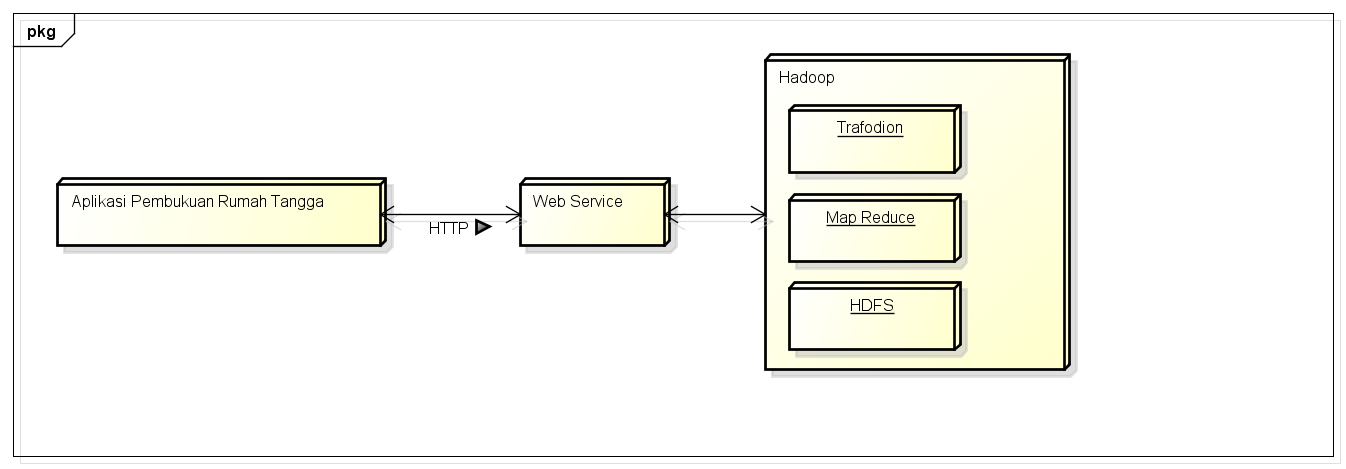
\includegraphics{Gambar/prt-architecture}
}
\caption[Permodelan Pembukuan Rumah Tangga]{Permodelan Pembukuan Rumah Tangga} 
\label{fig:prt_architecture}
\end{figure}

\section{Analisis Kebutuhan Perangkat Lunak}

\hspace{0,5cm}Pada sub-bab ini akan dibahas fitur-fitur yang disediakan aplikasi.

\subsection{Fitur Pada Aplikasi \textit{Mobile Device}}

\hspace{0,5cm}Pada aplikasi ini, terdapat beberapa peran, yaitu:
\begin{enumerate}
	\item Kepala rumah tangga
	\item	Pengurus rumah tangga
	\item Anggota rumah tangga
\end{enumerate}

Fitur-fitur yang ada, yakni:
\begin{enumerate}
	\item Pendaftaran diri, pendaftaran dilakukan untuk mendapatkan hak akses kedalam sistem aplikasi dan pendaftaran mendapat peran sebagai kepala rumah tangga
	\item Pengisian profil rumah tangga, pengisian profil dilakukan oleh kepala rumah tangga setelah mendaftarkan diri dan disetujui oleh admin
	\item	Mendaftarkan pengurus dan anggota rumah tangga, kepala rumah tangga dapat menambahkan dan mengurungai pengurus dan anggota rumah tangga yang berelasi terhadapnya
	\item Mencatat transaksi, semua peran mendapat hak akses untuk fitur ini dimana fitur ini untuk mencatat transaksi keuangan masing-masing.
	\item Alokasi keuangan, fitur ini berupa transfer dana antar anggota rumah tangga, baik dari kepala ke anggota dan sebaliknya, fitur ini hanya dimiliki oleh kepala dan pengurus rumah tangga.
	\item Menambah kategori transaksi, fitur ini hanya dimiliki oleh kepala rumah tangga yang bertujuan untuk menambah kategori transaksi.
	\item Melihat laporan keuangan, fitur ini hanya dapat diakses oleh kepala dan penguru rumah tangga.
	\item Melihat transaksi, fitur ini dapat diakses oleh semua peran rumah tangga.
\end{enumerate}

\subsection{Fitur Pada Aplikasi \textit{Website}}

\hspace{0,5cm}Aplikasi \textit{website} ini dibuat hanya untuk admin sehingga dapat mengatur data-data yang ada pada aplikasi.

Fitur-fitur yang ada yakni:
\begin{enumerate}
	\item Pengolahan anggota
				Admin dapat menyetujui atau menolak pendaftaran dari pengguna
	\item	Pengolahan kategori transaksi
				Admin dapat mengurangi atau menambah kategori transaksi
	\item Pelaporan
				Admin dapat membuat laporan secara keseluruhan
\end{enumerate}

\subsection{Diagram \textit{Use Case}}

\hspace{0,5cm}Diagram \textit{use case} oleh pengguna aplikasi dapat dilihat pada Gambar~\ref{fig:diagram_use_case_mobile}

\begin{figure}
\centering
\resizebox{\textwidth}{!}{
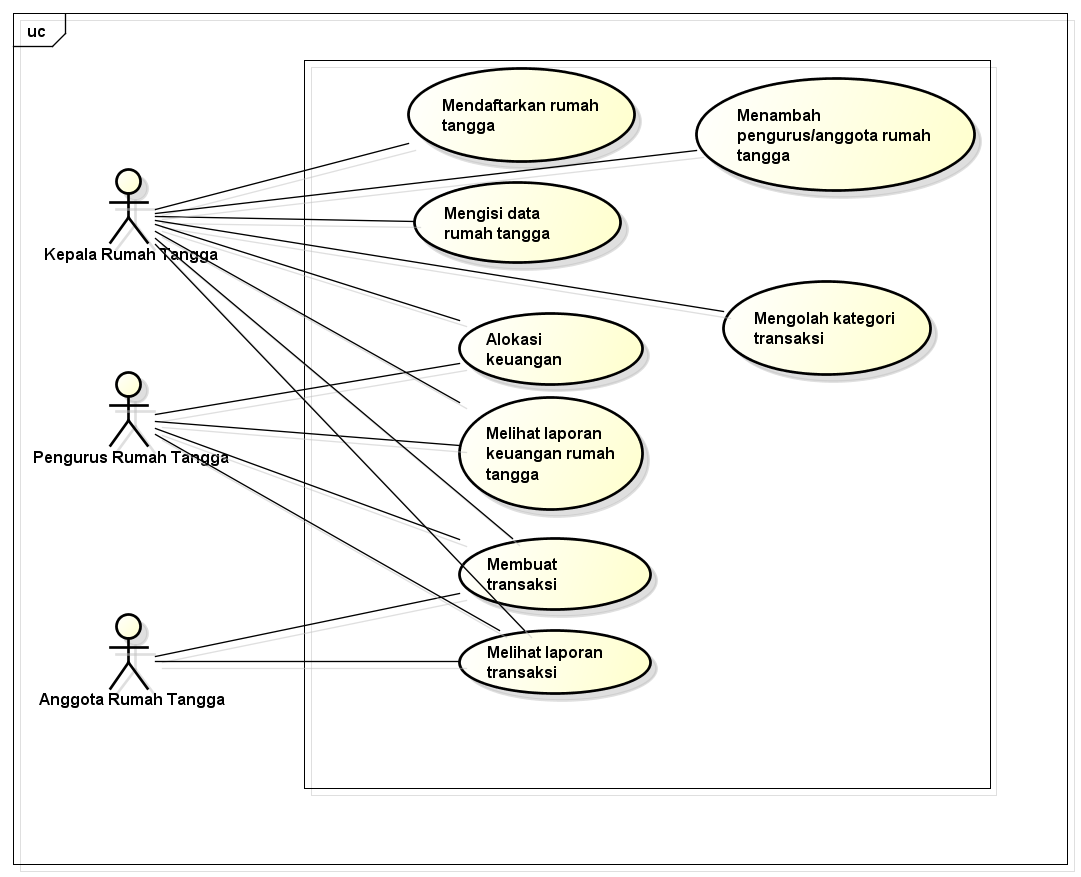
\includegraphics{Gambar/use-case-mobile}
}
\caption[Diagram \textit{Use Case Mobile Device}]{Diagram \textit{Use Case Mobile Device}} 
\label{fig:diagram_use_case_mobile}
\end{figure}

Diagram \textit{use case website} yang digunakan admin dapat dilihat pada Gambar~\ref{fig:diagram_use_case_website}

\begin{figure}
\centering
\resizebox{\textwidth}{!}{
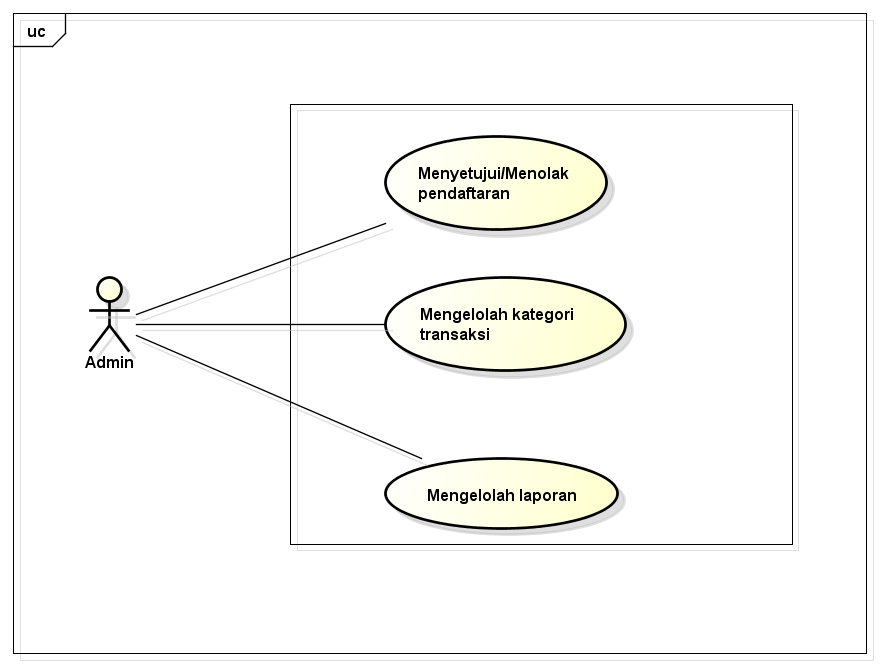
\includegraphics{Gambar/use-case-web}
}
\caption[Diagram \textit{Use Case Mobile Website}]{Diagram \textit{Use Case Mobile Website}} 
\label{fig:diagram_use_case_website}
\end{figure}